The problem of exploring an unknown territory is a fundamental problem in
robotics. The goal of exploration is to gain as much information as 
possible of the environment---through the robots' sensors---within bounded time. 
Applications of efficient exploration include search and rescue \cite{Kitano99robocuprescue}, planetary exploration \cite{apostolopoulos2001robotic} and military uses \cite{hougen2000miniature}.
The most common approach to exploration is based on \emph{frontiers}. A frontier
is a segment that separates known (explored) regions from unknown regions. By
moving towards frontiers, robots can focus their motion on discovery of new
regions. Yamauchi
\cite{yamauchi_frontier-based_1997,yamauchi_frontier-based_1998} was the first
to show a frontier-based exploration strategy. His work led to many
others (e.g,
\cite{burgard_collaborative_2000,burgard05tro,lau_behavioural_2003,sawhney_fast_2009}).

Investigations of single- and multi- robot frontier-based exploration all share
the key step of \textit{frontier detection}, which is the process that identifies
the current set of frontiers, given the current map (and/or history of the robots'
perceptions).  In almost all papers  base frontier detection on techniques borrowed from computer
vision: edge detection and region extraction (see Section~\ref{chap:related_work} for
a detailed discussion).  The frontiers need to be detected again and again, as
the exploration proceeds and areas that were once unknown become known.

To detect frontiers, existing methods process the entire map data with every execution to the algorithm.
As a result, as maps grow large, state-of-the-art frontier detection algorithms can 
take a number of seconds to run, even on powerful computers. This significantly
impacts the exploration strategy:  If a large region is 
explored, the robot actually has to wait in its
spot until the frontier detection algorithm terminates. Therefore, most
exploration implementations call the frontier detection algorithm only when the
robot arrives at its destination. Others do it only once some distance has 
been traveled, or once some time has passed since the last detection 
(see~\ref{chap:related_work} for details).
 
This slows down the exploration process, and can cause inefficiencies in the
exploration.
We present two examples:
First, consider a common \textit{single-robot case} (Figure~\ref{fig:single_example}),
where a robot exploring its environment detects a frontier and moves towards it (Figure~\ref{fig:single_1}).
Because of sensor coverage, the robot may in fact sense (and clear) all remaining unknown
area (Figure~\ref{fig:single_2}), but because it cannot call the
frontier-detection mechanism, it continues to move unnecessarily
(Figure~\ref{fig:single_3}). Similarly, consider a \textit{multi-robot case}
(Figure~\ref{fig:mutli_example}). Here, two robots,
 $R_1$ and $R_2$ which are located on bottom and top, respectively, 
are exploring the environment, from their initial locations (Figure~\ref{fig:multi_1}). 
One of the robots passes by a target assigned to the other, and thus clearing it
(Figure~\ref{fig:multi_2}).
But because the other robot cannot continuously re-detect frontiers, it unnecessarily continues
towards the covered target, instead of turning to more fruitful exploration targets.

\begin{figure}
 \centering
 \subfigure[ ] {
 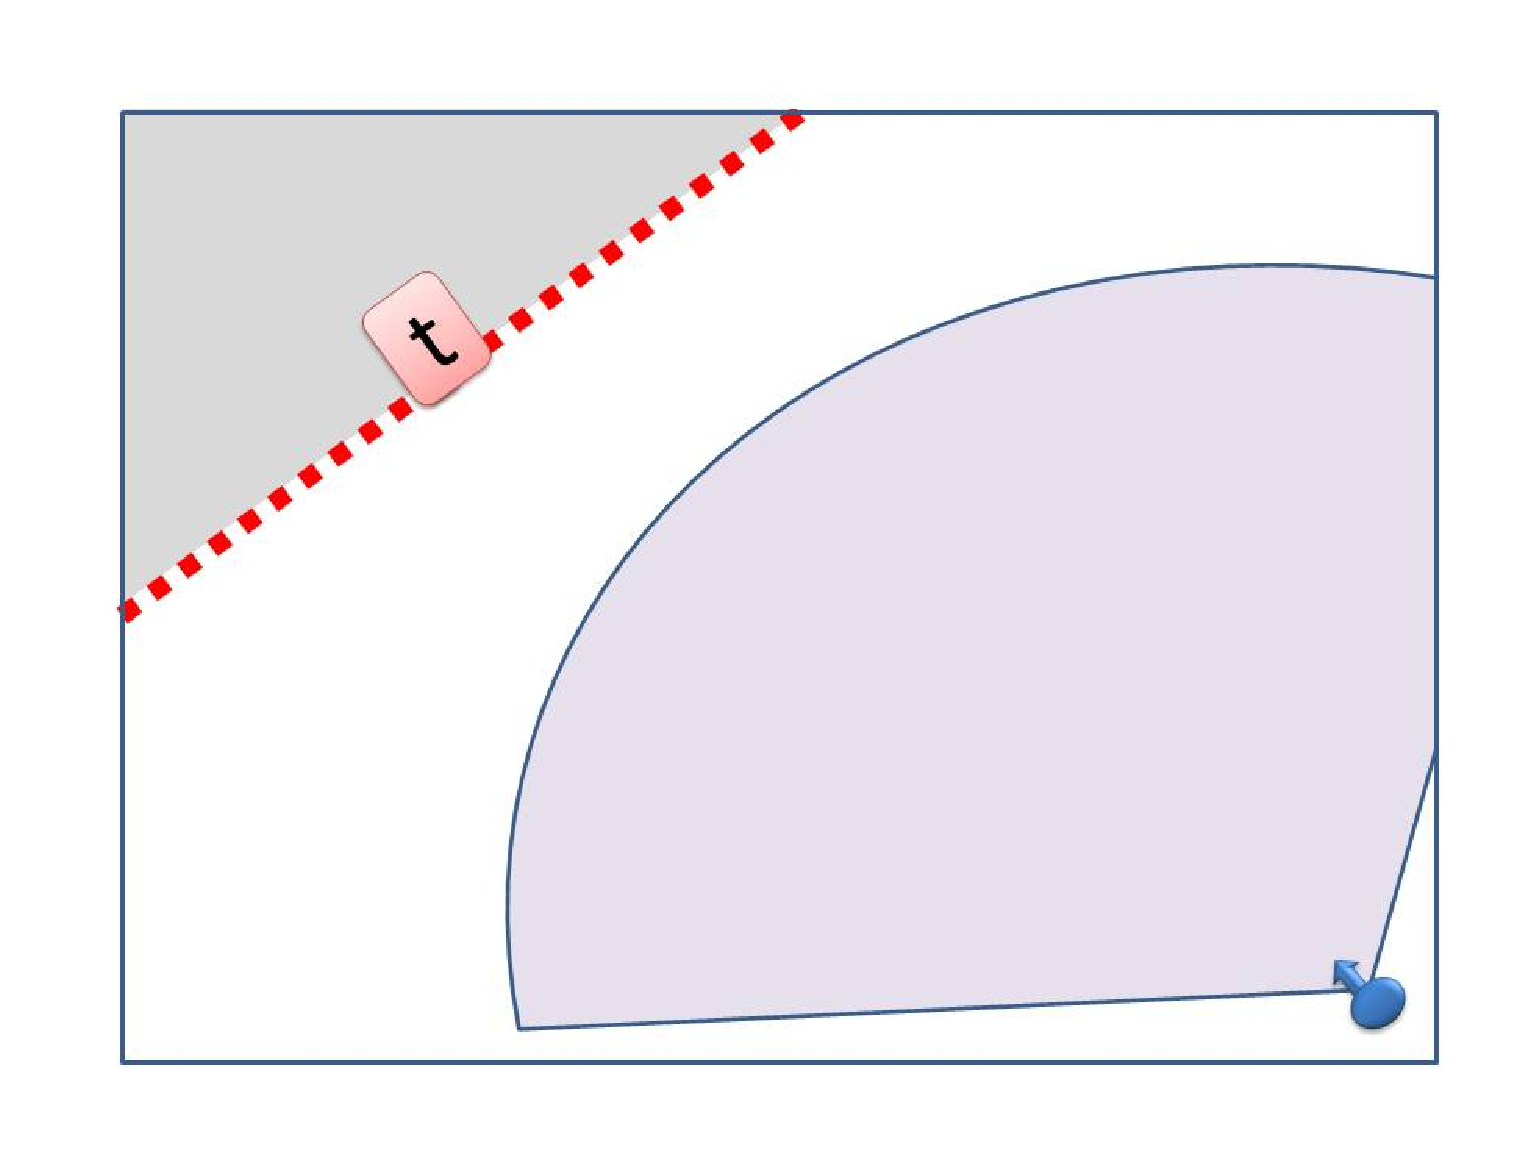
\includegraphics[width=0.3\columnwidth,keepaspectratio]{images/single_1}
 \label{fig:single_1}}
 \subfigure[ ] {
 \centering
 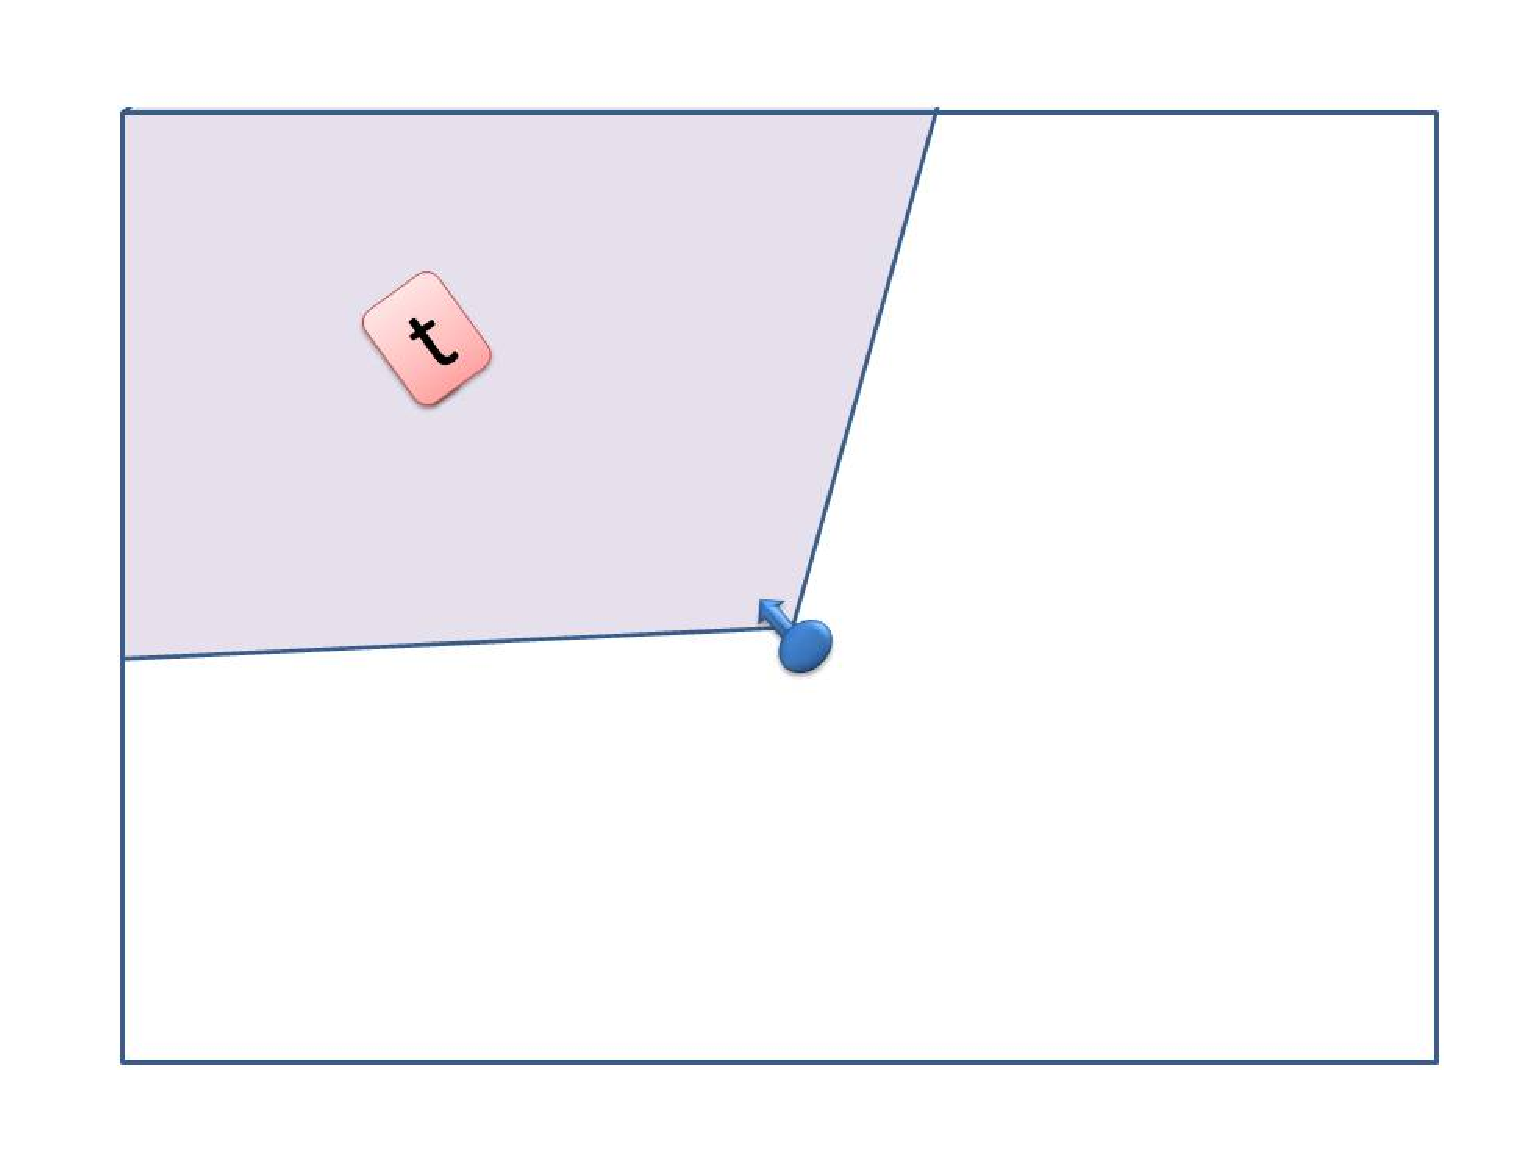
\includegraphics[width=0.3\columnwidth,keepaspectratio]{images/single_2}
 \label{fig:single_2}}
 \subfigure[ ] {
 \centering
 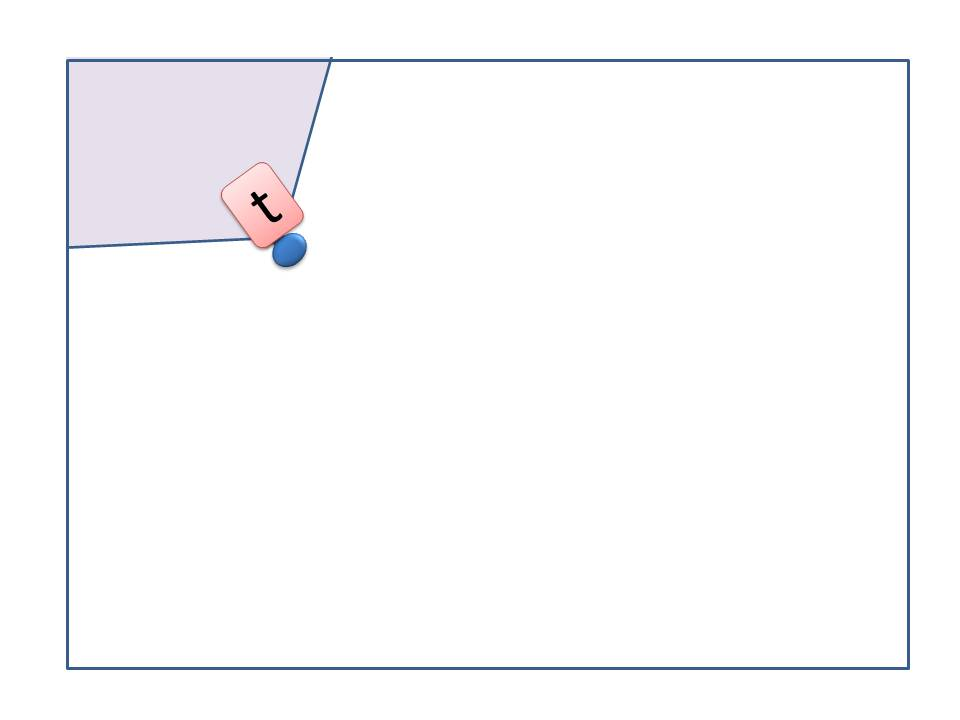
\includegraphics[width=0.3\columnwidth,keepaspectratio]{images/single_3}
 \label{fig:single_3}
 }
 \caption{A single-robot example. In 
 \ref{fig:single_1} the robot is heading towards the marked target on the frontier.  In 
 \ref{fig:single_2} the target and all of the remaining are covered by the robot's sensors, but because the robot does
  not re-detect frontiers, it continues to move.  In  \ref{fig:single_3} the robot has reached the frontier, unnecessarily.
 }
 \label{fig:single_example}
\end{figure}


\begin{figure}
 \centering 
 \subfigure[] {
 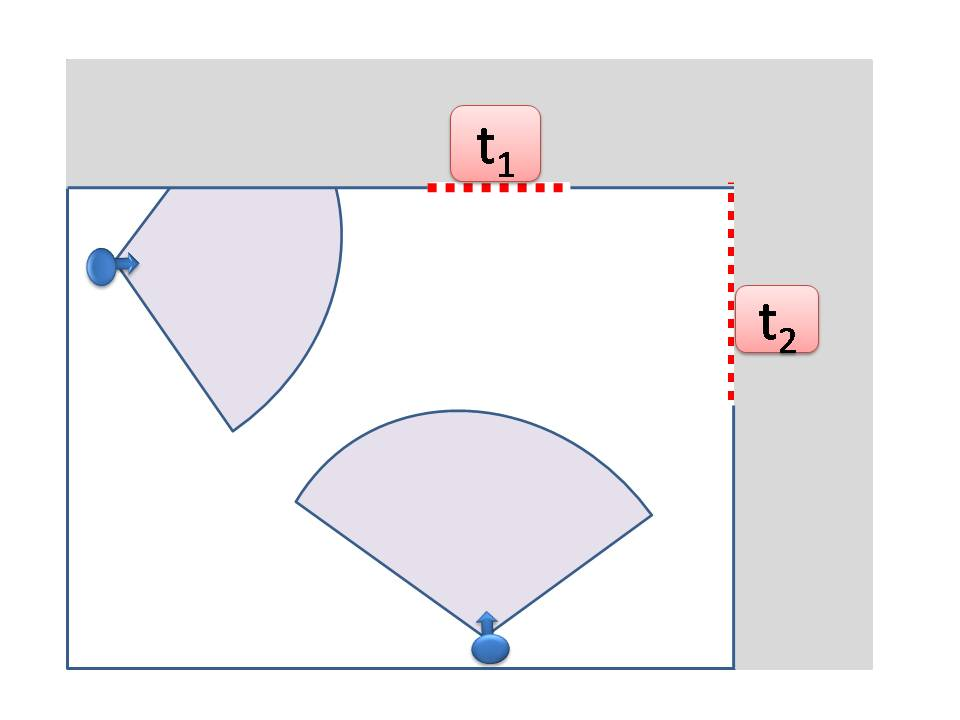
\includegraphics[width=0.45\columnwidth,keepaspectratio]{images/multi_1}
 \label{fig:multi_1}}
 \subfigure[] {
 \centering
 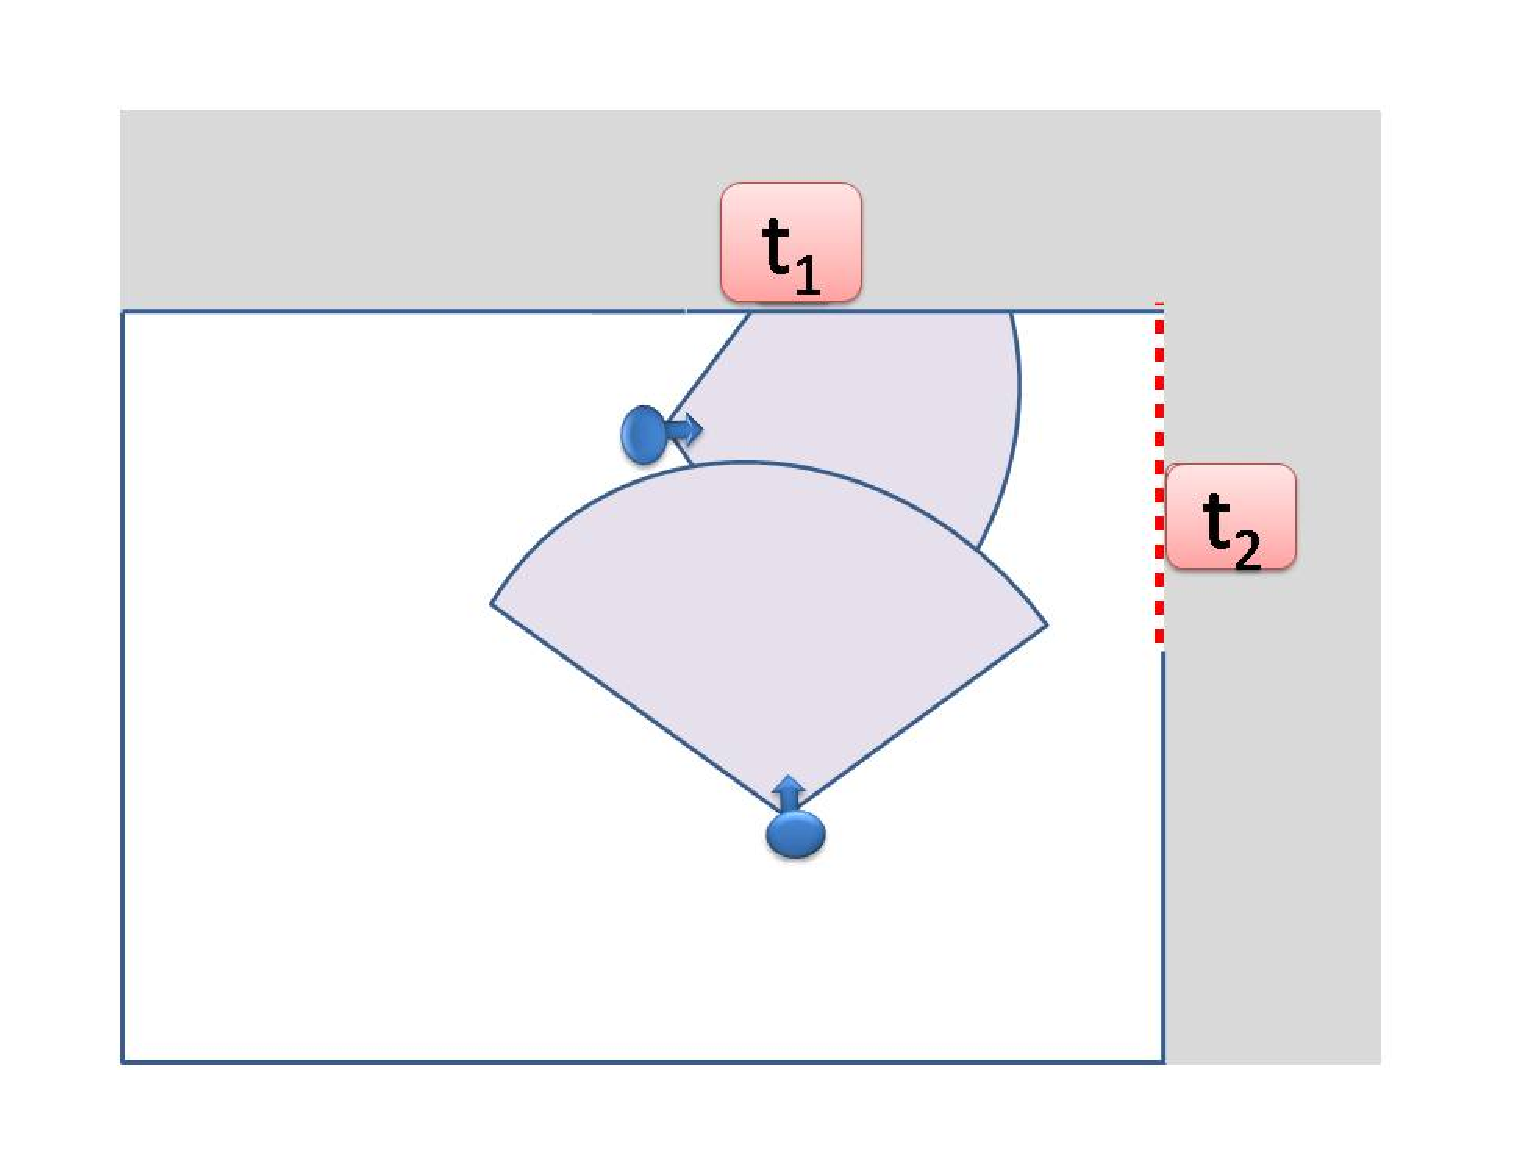
\includegraphics[width=0.45\columnwidth,keepaspectratio]{images/multi_2}
 \label{fig:multi_2}}
 \caption{A multi-robot example.  In~\ref{fig:multi_1}, the top robot ($R_2$) is heading towards the right target, $t_2$; the other robot ($R_1$) heads towards the top target $t_1$. In~\ref{fig:multi_2} $R_2$ has reached its target, clearing both $t_1$ and $t_2$, making $R_1$'s movements unnecessary.}
 \label{fig:mutli_example}
\end{figure}


In this work, we focus on significantly speeding up the frontier detection, common
to all frontier-based exploration techniques.
We introduce four algorithms for fast frontier detection.

The first, \WFD (Wavefront Frontier Detector) % (Section \ref{section:wfd})
is an iterative method that performs a graph-search over already-visited map
points (i.e., the known area), instead of the entire map (which includes also
unknown areas). It builds on ideas suggested in earlier
work~\cite{calisi2007multi} which were not evaluated as an
alternative to the edge-detection state-of-the-art. 
% The key idea in \WFD is that it does not scan the entire map, only the regions that have already been visited by the robot.
However, as exploration progresses, the scanned area grows, and thus \WFD cannot
be expected to perform well in large areas.  

Our second contribution is 
\FFD (Fast Frontier Detector), % (Section \ref{section:ffd}) is 
a novel approach for frontier detection which processes raw sensor readings,
and thus only scans areas that could contain frontiers. But because it works
with raw sensor data, it requires extending the evolving map with additional
data-structures, so that frontiers are maintained 
even when they are no longer within sensor range.
We describe these data-structures in detail, focusing on 
fast implementations.

Here's another way of looking at these algorithms. \WFD and edge-detection methods use the occupancy grid
maintained by a SLAM mapper as a representation of the accumulated, processed sequence $\langle
O_0,\ldots,O_t\rangle$. They thus essentially ignore most of the sequence, and
act (mostly) on the latest observation of the occupancy grid $G_t$, as it integrates all
sensor readings up to time $t$. The edge detection method processes $G_t$ (the
entire occupancy grid at time $t$). The \WFD algorithm processes a subset,
starting with the cell indicated by $P_t$ (the latest robot position), within
$G_t$.  \FFD uses $R_t$ (the latest range sensor readings) directly to detect current frontiers, and a modified
occupancy grid data structure to maintain/delete past frontiers.
We define these terms and notations formally in Section~\ref{section:definitions}. We then  
provide a theoretical complexity analysis for the algorithms,
and discuss their analytical correctness. 
% More definitions and terms related to the frontier detection problem can be
% found in Section \ref{section:definitions}.

Finally, we synthesized the different approaches of \WFD and \FFD into two 
novel algorithms: \WFDINC and \WFDIP. Both algorithms
perform frontier detection on known regions but they differ from \WFD by
searching for frontiers only within the areas that were covered by the robot
sensors since last call. They thus borrow from \FFD the ability to maintain
knowledge of frontiers not currently visible.


We provide a detailed evaluation of all algorithms, and contrast them 
with the state-of-the-art (\SOTA). % (in Section
% \ref{section:experimental_results}.
Specifically, we examine their performance in different types of environments,
 and on two different CPUs. We show that \WFD and \WFDINC are faster than \SOTA by 1--2 orders of
magnitude, and that \FFD and \WFDIP are faster than \WFD and \WFDINC by 
additional 1--2 orders of magnitude.  The results make it possible to execute real-time
frontier-detection on current-day robot CPUs, opening the way to novel
frontier-based exploration strategies which were impractical until now.
